
\begin{figure*}[ht]
\centering
%\includegraphics[width=3.5in]{pics/system_architecture.eps}
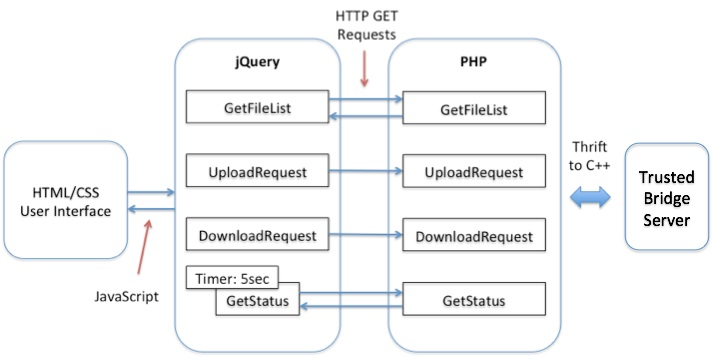
\includegraphics[width=5.2in]{pics/web_arch.png}
\caption{Front-end web server architecture.}
\label{fig:web}
\end{figure*}

Trusted Bridge has an elegant web user interface to provide the user with an intuitive click-and-go file upload and download accessibility. The front-end web service is composed of three
components: HTML/CSS for the interface template, JavaScript/jQuery for UI logic control, and PHP for handling file upload and download from client browsers. Figure~\ref{fig:web} shows the architecture of the front-end web server.

We use Twitter Bootstrap to rapidly build the web user interface. Bootstrap contains HTML and CSS-based design templates for typography, forms, buttons, navigation and other interface components, as well as some useful JavaScript extensions. The HTML/CSS contents will be automatically updated to reflect the current system status including the error message from Trusted Bridge server, the change of file list, upload and download progress, and etc. 

With the help of jQuery, we could easily modify the HTML/CSS DOM objects dynamically. The UI event will trigger callback functions written in jQuery and do the related action. All the requests will be forwarded to a PHP program, which could arbitrarily access files on web server with appropriate permissions. The PHP program will talk to Trusted Bridge server through Apache Thrift protocol.

For example, when the user click on "Add File" button, a file selector will pop out. After the file selection by the user, the file upload event in jQuery will be triggered and send the selected file from user's local storage to web server temporary folder. The PHP program will handle the upload request and send the file location to Trusted Bridge server. After the file partitioning and uploading to external cloud storage, Trusted Bridge server will response a OK message. The PHP program will just pass this response to front-end JavaScript with JSON format. When the front-end get the response, it will call GetFileList to get the latest file list in the system.

For downloading files, when the user click on the download button right next to the file name, jQuery will send a HTTP request to PHP server to ask for download action. The PHP program then forward the request to Trusted Bridge server through Thrift. After the file assembling task is finished, a downloadable intact will be saved in web server temporary folder. The front-end jQuery will check whether the file is ready or not every five seconds with the help of PHP server. Once the file is ready, the requested file will be automatically downloaded into user's local disk.
